\let\negmpace\undefined
\let\negthickspace\undefined
\documentclass[journal]{IEEEtran}
\usepackage[a5paper, margin=10mm, onecolumn]{geometry}
%\usepackage{lmodern} % Ensure lmodern is loaded for pdflatex
\usepackage{tfrupee} % Include tfrupee package
\setlength{\headheight}{1cm} % Set the height of the header box
\setlength{\headsep}{0mm}     % Set the distance between the header box and the top of the text
\usepackage{gvv-book}
\usepackage{gvv}
\usepackage{cite}
\usepackage{amsmath,amssymb,amsfonts,amsthm}
\usepackage{algorithmic}
\usepackage{graphicx}
\usepackage{textcomp}
\usepackage{xcolor}
\usepackage{txfonts}
\usepackage{listings}
\usepackage{enumitem}
\usepackage{mathtools}
\usepackage{gensymb}
\usepackage{comment}
\usepackage[breaklinks=true]{hyperref}
\usepackage{tkz-euclide} 
\usepackage{listings}
% \usepackage{gvv}                                        
\def\inputGnumericTable{}                                 
\usepackage[latin1]{inputenc}                                
\usepackage{color}                                            
\usepackage{array}                                            
\usepackage{longtable}                                       
\usepackage{calc}                                             
\usepackage{multirow}                                         
\usepackage{hhline}                                           
\usepackage{ifthen}                                           
\usepackage{lscape}
\renewcommand{\thefigure}{\theenumi}
\renewcommand{\thetable}{\theenumi}
\setlength{\intextsep}{10pt} % Space between text and floats
\numberwithin{equation}{enumi}
\numberwithin{figure}{enumi}
\renewcommand{\thetable}{\theenumi}
\title{Assignment3}
\author{Teja Vardhan Shannu}
\date{August 2024}

\begin{document}
\maketitle
\textbf{Problem:} A line intersects the Y-axis and the X-axis at the points $P(0,b)$ and $Q(c,0)$ respectively. If $(2,-5)$ is the midpoint of $PQ$, then find the coordinates of $P$ and $Q$.

\textbf{Solution:}

Let the coordinates of points $P$ and $Q$ be represented by the vectors:
\begin{align}
	\mathbf{P} = \begin{pmatrix} 0 \\ b \end{pmatrix}, \quad \mathbf{Q} = \begin{pmatrix} c \\ 0 \end{pmatrix}
\end{align}
The midpoint $M$ is given as:
\begin{align}
       \mathbf{M} = \begin{pmatrix} 2 \\ -5 \end{pmatrix}
\end{align}	
The midpoint formula in vector form is:
\begin{align}
       \mathbf{M} = \frac{1}{2} (\mathbf{P} + \mathbf{Q})
\end{align}
Substituting the given values:
\begin{align}
       \frac{1}{2} \left(\begin{pmatrix} 0 \\ b \end{pmatrix} + \begin{pmatrix} c \\ 0 \end{pmatrix}\right) = \begin{pmatrix} 2 \\ -5 \end{pmatrix}
\end{align}
This simplifies to:
\begin{align}
       \frac{1}{2} \begin{pmatrix} c \\ b \end{pmatrix} = \begin{pmatrix} 2 \\ -5 \end{pmatrix}
\end{align}
Multiplying both sides by 2:
\begin{align}
       \begin{pmatrix} c \\ b \end{pmatrix} = \begin{pmatrix} 4 \\ -10 \end{pmatrix}
\end{align}
Thus, the coordinates of $P$ and $Q$ are:
\begin{align}
       \mathbf{P} = \begin{pmatrix} 0 \\ -10 \end{pmatrix}, \quad \mathbf{Q} = \begin{pmatrix} 4 \\ 0 \end{pmatrix}
\end{align}

\begin{figure}[ht!]
  \hspace{-3cm}
  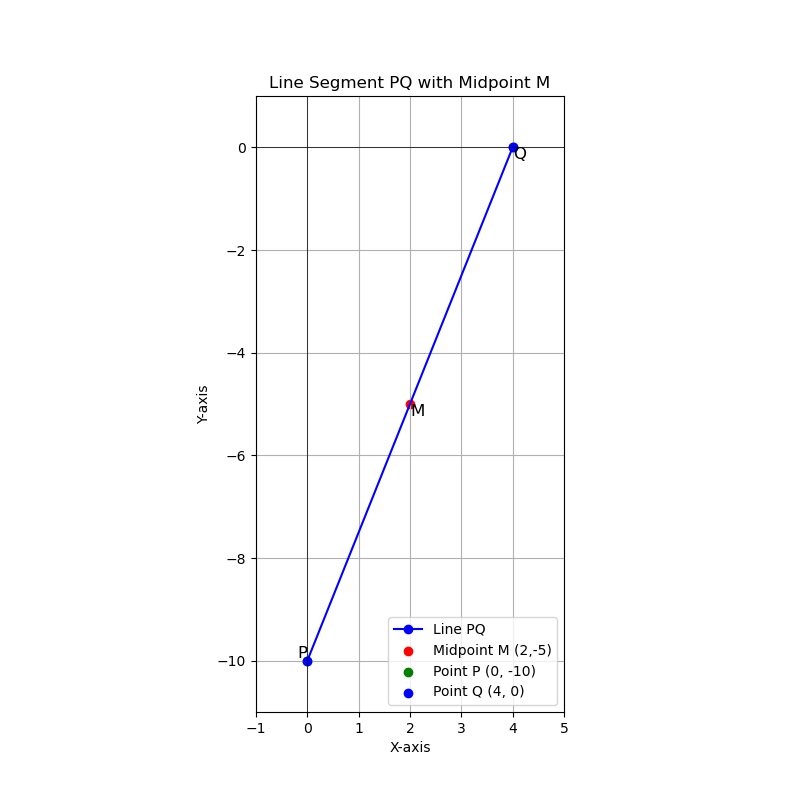
\includegraphics[width=1.5\textwidth]{Figure_1.png}
  
  \caption{The plot of the points }
  \label{fig:your_label}
\end{figure}

\end{document}

